\begin{tframe}{Dataset Creation}

The phase for the \textbf{dataset creation} consists in the acquisition of images exploiting the modern \textit{image search engines}.

\vspace{0.1in}

It is necessary to decide a list of \textbf{identities} that are sufficiently popular, so that for each identity there will be a high number of images (between 500 and 1000), as results of the search engines.

\vspace{0.1in}

The acquisition procedure is divided in two parts: 

\begin{itemize}
\item A collection phase.
\item A download phase.
\end{itemize}

\end{tframe}

\begin{tframe}{Dataset Creation}

The \textbf{collection} phase takes advantage of three search engines, such as Bing, Yahoo and AOL, to query and obtain images for each identity.

\vspace{0.1in}

A query to an image search engine returns a HTML page; thanks to a parser, implemented for each search engine, we can obtain the links to the images contained in each HTML page.

\begin{figure}[h]
\centering
\hspace*{\fill}
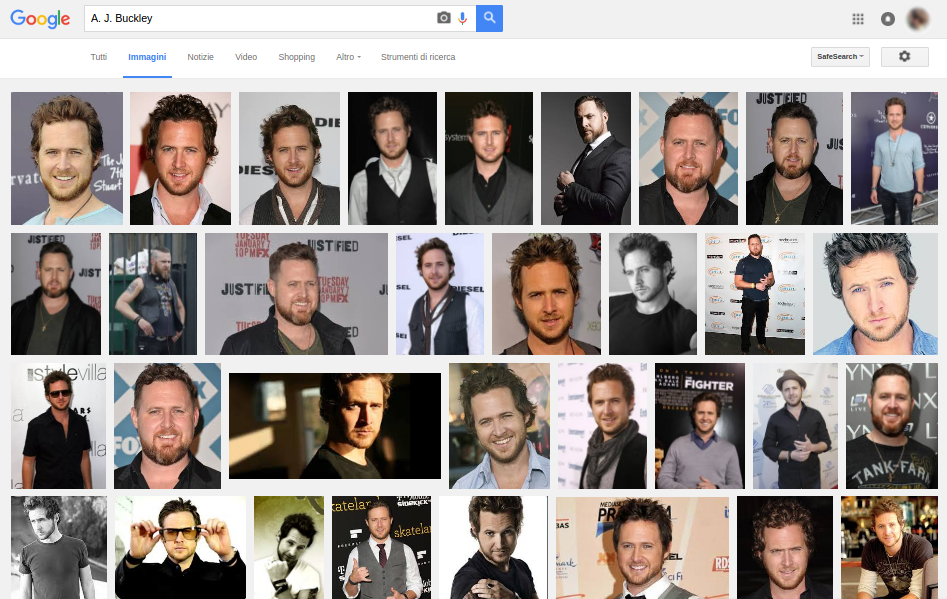
\includegraphics[width=0.40\textwidth]{images/image8.png}
\hspace*{\fill}
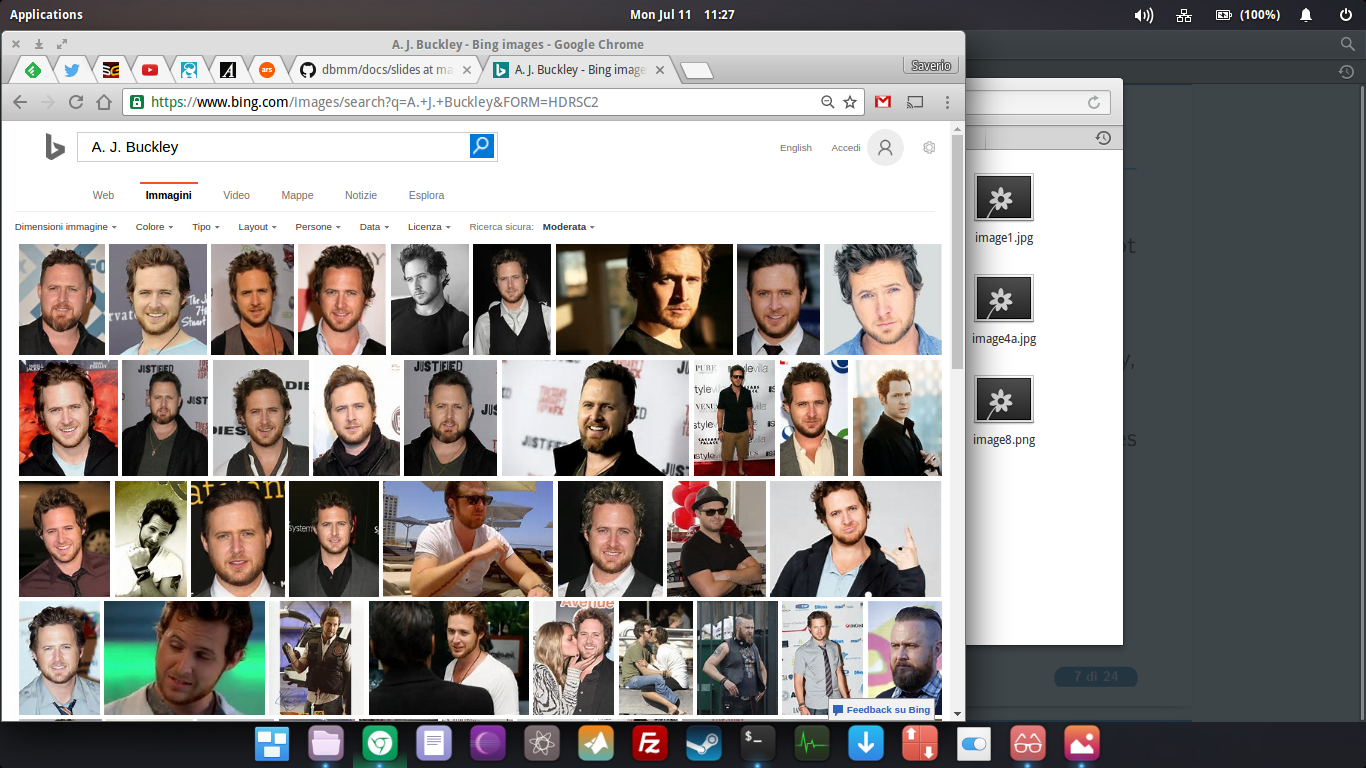
\includegraphics[width=0.40\textwidth]{images/image11.png}
\hspace*{\fill}
\end{figure}


The \textbf{download} phase is straight forward: the images are downloaded and saved in a folder related to the identity, using the links obtained in the previous step.

\end{tframe}